\chapter{Исследовательский раздел}
В данном разделе представлены технические характеристики компьютера, используемого для тестирования и экспериментов, и примеры работы программы.
 \section{Технические характеристики}

Ниже приведены технические характеристики устройства, на котором были проведены эксперименты при помощи разработанного ПО:

\begin{itemize}
	\item операционная система: Windows 10 (64-разрядная);
	\item оперативная память: 32 GB;
	\item процессор: Intel(R) Core(TM) i7-7700K CPU @ 4.20GHz;
	\item количество ядер: 4;
	\item количество потоков: 8.
\end{itemize}

\section{Примеры работы программы}
На рисунках \ref{results1}-\ref{results2} представлены примеры работы программы.

\begin{figure}[h]
	\center{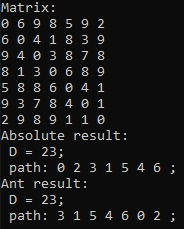
\includegraphics[width=0.3\linewidth]{inc/img/results1}}
	\caption{Результат работы программы}
	\label{results1}
\end{figure}

\begin{figure}[h]
	\center{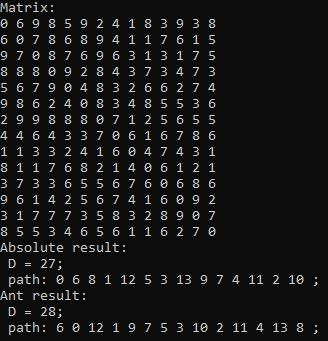
\includegraphics[width=0.6\linewidth]{inc/img/results2}}
	\caption{Результат работы программы}
	\label{results2}
\end{figure}

\section{Постановка экспериментов}

Проведем эксперимент, чтобы установить при каких параметрах муравьный алгоритм работает лучше всего. Возьмем значения ro от 0 до 1 с шагом 0.25, значения alpha от 0 до 1 с шагом 0.25 и значения Tmax от 50 до 400 с шагом 50.

На рисунке \ref{times} представлены результаты эксперимента. В первых трех столбцах находятся значения ro, alpha и tmax соответственно. В четвертом столбце находится среднее максимальное отклонение при данных параметрах. 
Замеры проводились для матрицы 12х12, также предварительно был высчитан идеальный путь с помощью алгоритма полного перебора.

\begin{figure}[h]
	\center{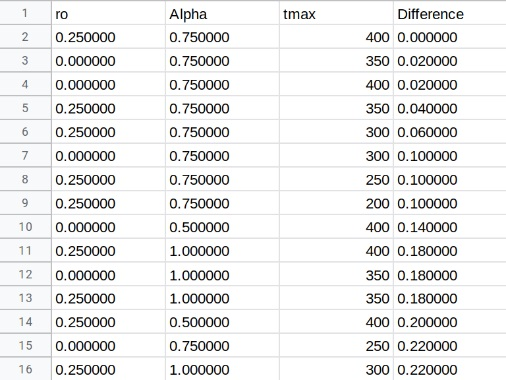
\includegraphics[width=1\linewidth]{inc/img/times}}
	\caption{Результат эксперимента с изменением параметров}
	\label{times}
\end{figure}

\newpage
По полученным данным можно сделать вывод, что алгоритм лучше всего работает на значениях ro от 0 до 0.25 и alpha от 0.75 до 1 при tmax от 350 до 400.

Далее проведем замеры по времени для муравьиного алгоритма с параметрами ro=0.25, alpha=0.75, tmax = 350 и для алгоритма полного перебора.

Для произведения замеров времени выполнения реализаций алгоритмов будет использована формула $t=\frac{T_{n}}{N}$, где N – количество замеров, t – время выполнения реализации алгоритма, Tn — время выполнения N замеров. Неоднократное измерение времени необходимо для построения более гладкого графика и получения усредненного значения времени.

Количество замеров будет взято равным 50. Замеры проводятся для матриц размером от 2 до 15 элементов.

На рисунке \ref{graphics} представлены результаты эксперимента.

\begin{figure}[h]
	\center{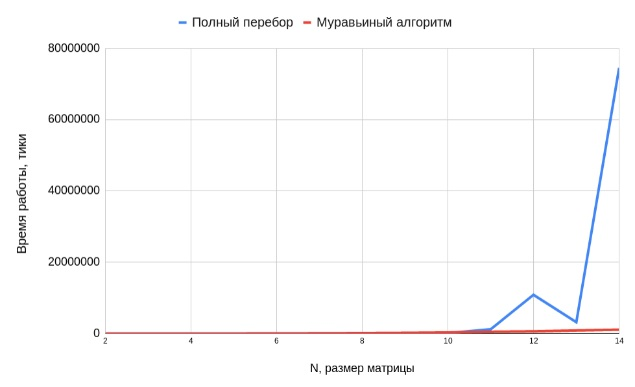
\includegraphics[width=1\linewidth]{inc/img/graphics}}
	\caption{Зависимость времени работы алгоритмов от размера матрицы}
	\label{graphics}
\end{figure}

\begin{figure}
	\begin{tikzpicture}
		\begin{axis}[
			%title={Зависимость времени выполнения алгоритмов LenLev() и LenLevRecCash() от длины слов},
			xlabel={N, размер матрицы},
			ylabel={Время выполнения, тики},
			xtick={2,3,4,5,6,7,8,9,10,11,12,13,14},
			legend pos=north west,
			ymajorgrids=true,
			grid style=dashed,
			width = 400
			]
			
			\addplot[
			color=blue,
			mark=square,
			]
			coordinates {
				(2,0)(3,0)(4,0)(5,0)(6,0)(7,0)(8,2)(9,16)(10,105)(11,224)(12,1603)(13,4643)(14,2600)
			};
			\addlegendentry{Полный перебор}
			
			
			\addplot[
			color=red,
			mark=square,
			]
			coordinates {
				(2,0)(3,3)(4,8)(5,18)(6,33)(7,56)(8,91)(9,147)(10,220)(11,313)(12,434)(13,567)(14,747)
			};
			\addlegendentry{Муравьинный алгоритм}
			
		\end{axis}
	\end{tikzpicture}
	\caption{Зависимость времени работы алгоритмов от размера матрицы}
	\label{graphics2}
\end{figure}

\clearpage
По рисунку видно, что алгоритм полного перебора  работает гораздо медленнее, чем муравьиный алгоритм, начиная с матрицы размером 10х10 и далее.

\section{Вывод}
По итогу иследования выяснилось, что разработанный алгоритм работает верно, то есть находит самый длинный полиндром в строке. Кроме этого был проведён анализ и сделан вывод по логу программы.

В ходе экспериментов было вычислены параметры муравьиного алгоритма, при которых результат наиболее приближен к идеальному. При увеличении параметра $t_{max}$ возрастает вероятность найти оптимальное решение, однако возрастает и время работы программы. По скорости муравьиный алгоритм сильно выигрывает у алгоритма полного перебора, на матрицах, размер которых превышает 10х10. Алгоритм полного перебора следует использовать на матрицах меньшего размера или в задачах, где требуется гарантировано точное решение.